\section{Experiments}
\label{sec:exp}

\begin{figure}
    \centering
    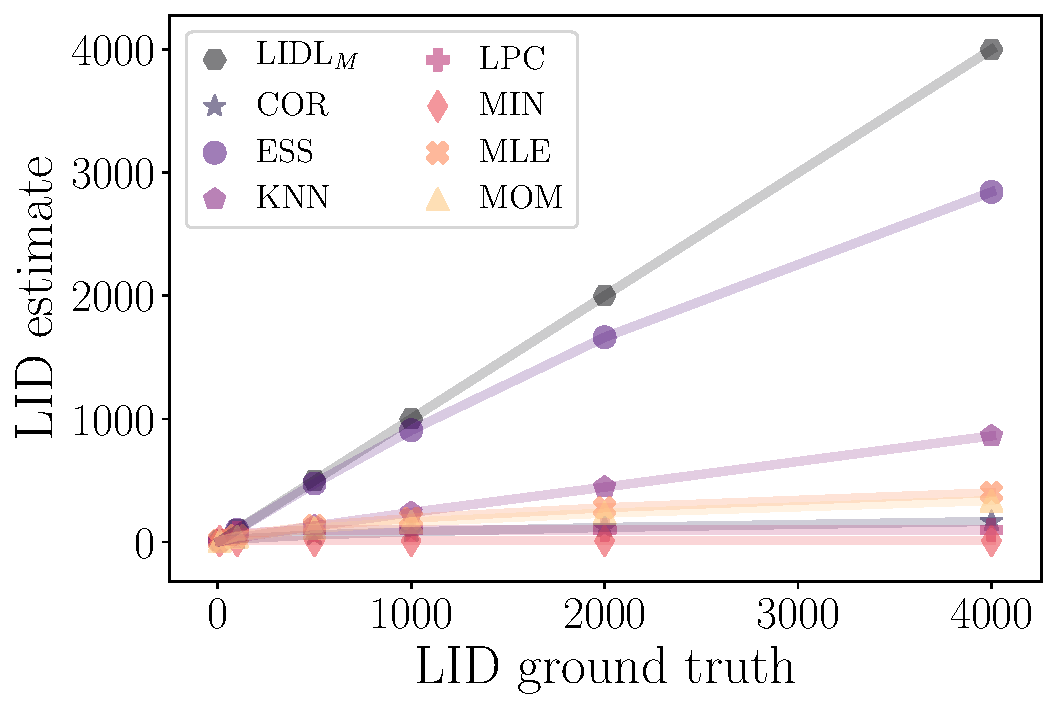
\includegraphics[width=0.45\textwidth]{images/uniform-scalability.pdf}
    \caption{LID estimates for $d$ dimensional uniform distribution on a hypercube. More results and abbreviation explanations can be found in Tables~\ref{tab:comparison},~\ref{tab:comparison-mae}~and~\ref{tab:skdim} in Appendix~\ref{sec:exp-details}.  The dimensionality $d$ of the distribution is plotted on the horizontal axis and the estimates for different algorithms on the vertical axis.}
    \label{fig:uniform-scalability}
\end{figure}

In this section, we compare LIDL with other algorithms, investigate its behavior with imperfect density estimators, and run it on real-world datasets. Details of training procedure can be found in Appendix~\ref{sec:exp-details} and in Sec.~\ref{sec:exp-reducing} we describe how to reduce an error of our estimate.

\subsection{Comparison on synthetic datasets}

We collated LIDL with other LID estimation algorithms from \texttt{scikit-dimension} Python library \citep{e23101368}, which covers all of the important algorithms for LID estimation, and compared them in three different aspects: %
\emph{1}.\ Scalability, 
\emph{2}.\ Multidimensional and curved manifolds,
\mbox{\emph{3}.\ Multiscale manifolds}.


We excluded FisherS and DANCo algorithms because they do not scale well to higher-dimensional settings. FisherS suffered from memory problems on medium datasets, and DANCo had unfeasibly long runtimes (multiple weeks) on the thousand-dimensional datasets.
According to the convention in the field, we choose to make comparison only on synthetic datasets, because we have ground truth for them.


\begin{figure}
    \centering
    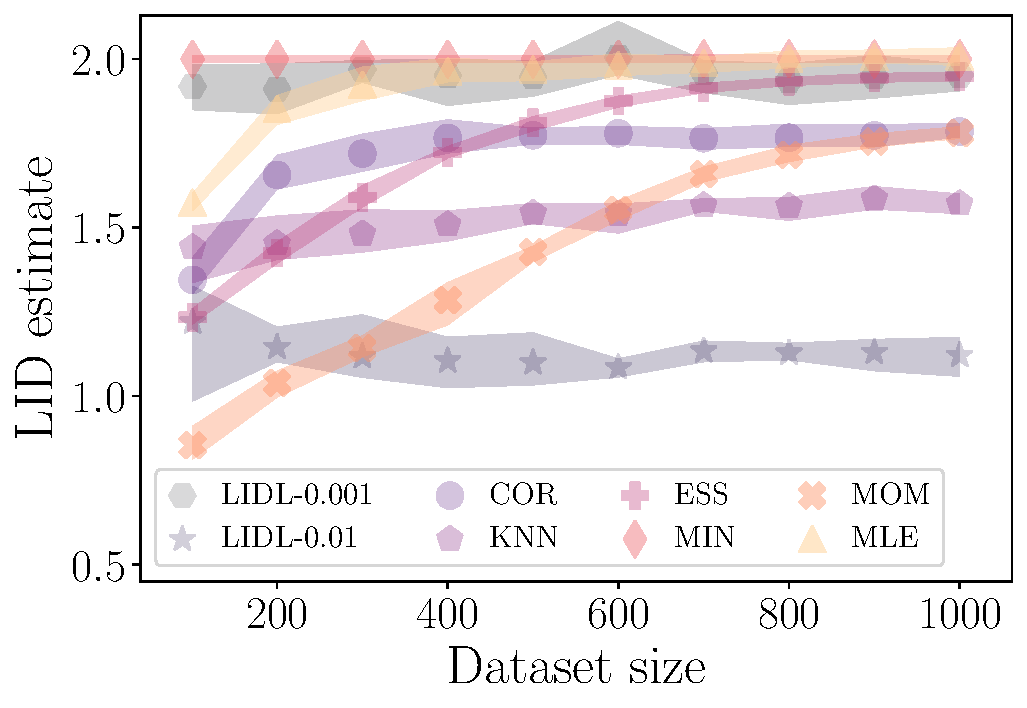
\includegraphics[width=0.44\textwidth]{images/multiscale-comparison.pdf}
    \caption{LID estimates for uniform distribution on a rectangle with edge lengths equal to 0.1 and 0.01. The size of the dataset is plotted on the horizontal axis and the estimate (with respective 95\% confidence intervals) on the vertical axis. For most algorithms (except LIDL, KNN and MIN), we can see a disturbing phenomenon: the estimate depends on the sample size. LIDL-$\delta$ stands for LIDL with MAF density estimator and scale parameter $\delta$.Other abbreviations are explained in appendix in Table~\ref{tab:skdim}.}
    \label{fig:multiscale-comparison}
\end{figure}

\paragraph{Scalability}

To test scalability we ran all algorithms on standard multidimensional uniform and normal distributions up to 4K dimensions. Detailed results of the comparison are gathered in Appendix~\ref{sec:exp-details} in Tables~\ref{tab:comparison} and \ref{tab:comparison-mae} (starting from the 7-th row). Each dataset consisted of 10K data points and each algorithm was run 5 times on different samples from the distribution. For each run, we calculated differences between true LID and estimate and averaged it over 5 runs. Then we divided the result by the average manifold dimensionality for each dataset, getting a relative bias of each algorithm. In subsequent tables, we report relative MAE and estimate standard deviation for the same procedure. 
From those tables, we can clearly see, that although in many cases LIDL does not have the lowest error and bias, for almost all datasets the results are in the $\pm5\%$ range. Other algorithms fail to accurately estimate dimensions exceeding 100. One exception is ESS, which stands out from the rest but remains inferior to LIDL. We plot LID estimates for some of the algorithms (we omitted few for the sake of clarity) for multidimensional uniform distributions in Fig.~\ref{fig:uniform-scalability}. All the abbreviations used in the plot are explained in Appendix~\ref{sec:exp-details}.

\begin{figure}[t]
    \centering
    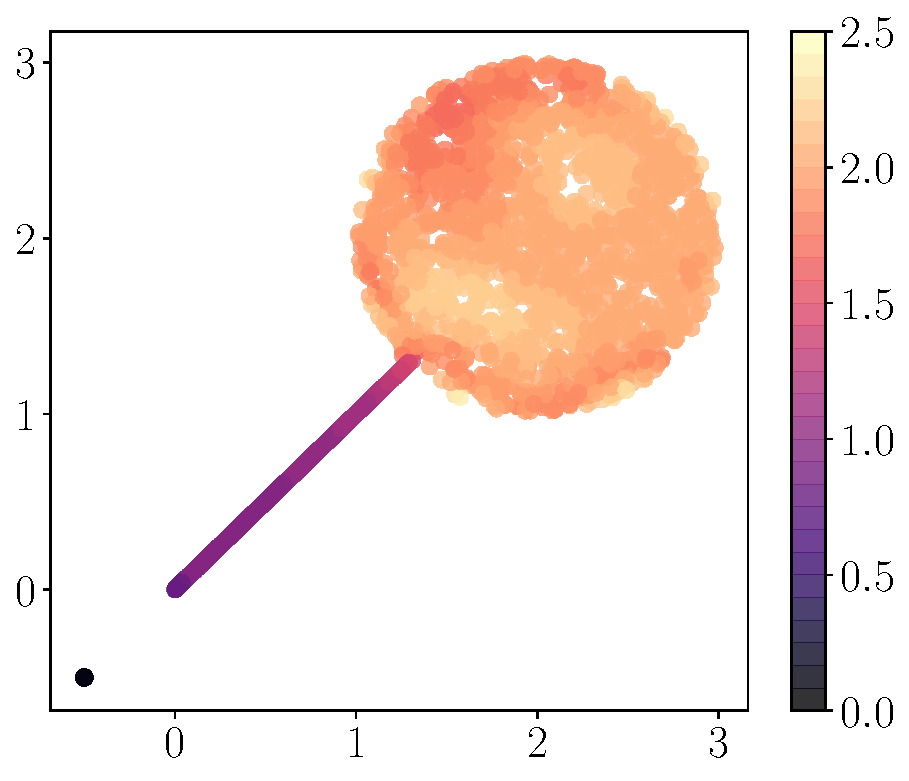
\includegraphics[width=0.49\textwidth]{images/maf-lollipop.pdf}
    \caption{Points from the lollipop benchmark dataset and LIDL (with MAF) estimates for those points.}
    \label{fig:maf-lollipop}
\end{figure}



\paragraph{Multiscale manifolds}
In the Introduction, we postulated that a useful LID estimation algorithm should operate properly on multiscale manifolds. 
In this section, we compare existing LID methods and LIDL on highly non-isotropic datasets. 
We observed that most of the algorithms with the same scale parameters (or those without such parameters, like ESS) give different results for different sizes of the dataset. 
We hypothesize that this may be caused by violating assumptions about the local uniformity of the distribution, but we did not investigate it further. 
Only LIDL, MiND\-ML, DANCo, and KNN give stable estimates for different dataset sizes. 
We plot those results for selected algorithms in Fig.~\ref{fig:multiscale-comparison}. For both scale parameter values, LIDL gives stable estimates for different dataset sizes. 
The rest of the unplotted algorithms also give unstable estimates, and we omitted them only to make the plot more readable. 


\paragraph{Curved manifolds and unions of manifolds}

We tested LIDL and other algorithms on some smaller but more complicated manifolds. We used three classical benchmarks from \cite{kleindessner2015dimensionality}: the Swiss roll dataset, uniform density on a helix, and uniform density on a sphere. These datasets lie on a curved manifolds (2-, 1- and 7-dimensional respectively) which may cause difficulties with fitting density estimators. Results of those experiments can be found in rows 4-7 of Tables~\ref{tab:comparison} and \ref{tab:comparison-mae}. The results for LIDL are decent (Relative bias less than 0.05 and relative MAE less than 0.06), but lPCA and ESS gave estimates with relative bias and MAE less than 0.01. For perfect density estimates LIDL gives almost perfect estimates on those datasets, as presented in Sec.~\ref{sec:other-perfect-datasets}.

None of the above datasets however consisted of components of different dimensions, which may be the case for many real-world datasets. We used a \emph{lollipop dataset}, which is composed of 0, 1, and 2-dimensional components. The dataset and its corresponding LIDL estimates are plotted in Fig.~\ref{fig:maf-lollipop}. On the 2- and 1-dimensional parts, many algorithms achieved good results, some even better than LIDL, but the 0-dimensional component, which consisted of replicas of the same point, caused most problems for other algorithms. 

When algorithms tried to estimate LID for this 0-dimensional part, only lPCA and LIDL were able to estimate its dimensionality properly, and almost all other algorithms failed to converge. When we jittered those points a little with $\N(0,10^{-6})$, almost all of the algorithms converged but all of them yielded estimates close to 2. Thanks to the possibility of setting operating scale in LIDL, we could estimate the latter dimension correctly, regardless of noise in the data. Results for each component of the manifold treated separately can be found in the first 3 rows of Tables~\ref{tab:comparison} and \ref{tab:comparison-mae}.

\subsection{Operating range}
\label{sec:operating-range}
As stated in Sec.~\ref{sec:scale}, $\delta$ can be seen as a scale parameter. We introduced some numerical and theoretical results to support this hypothesis, and in this section, we are going to present some experiments investigating this topic. In Fig.~\ref{fig:step-delta-uniform} we present a similar experiment to that from Fig.~\ref{fig:step-delta-exp}, but this time with 4-dimensional uniform density. Results seem quite similar to previous theoretical results. For similar Gaussian distribution, we get an almost identical relation between dimension variance, LIDL estimate and $\delta$.

We also tuned a $\delta$ range on image MNIST and FMNIST to reduce dequantization noise influence on the LIDL estimate. More on those experiments can be found in Appendix~\ref{sec:exp-details}. Although this scale parameter has to be used with care. In one experiment on FMNIST (normalized to have values between -0.5 and 0.5) for values of $\delta > 0.1$ we observed that the whole cluster of darker clothes had been estimated as being 0-dimensional. We present some samples from this cluster in Fig.~\ref{fig:dark}.

\begin{figure}[t]
    \centering
    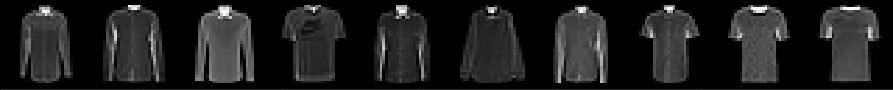
\includegraphics[width=\linewidth]{images/dark-shirts.png}
    \caption{Images from the FMNIST dataset, for which the LID estimate is close to 0. This effect occurred when we used to high $\delta$s for this thin data manifold.}
    \label{fig:dark}
\end{figure}


\subsection{Experiments on image datasets}

\begin{figure}[b]
    \centering
    \newcommand\figwidth{0.16\textwidth}
    \minipage{\figwidth}
    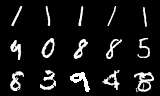
\includegraphics[width=0.99\textwidth]{images/mnist.png}
    \endminipage
    \minipage{\figwidth}
    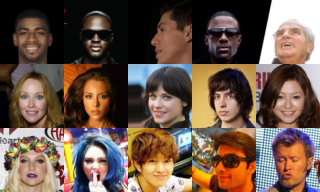
\includegraphics[width=0.99\textwidth]{images/celeba.png}
    \endminipage
    \minipage{\figwidth}
    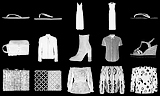
\includegraphics[width=0.99\textwidth]{images/fmnist.png}
    \endminipage
    \caption{Samples from different image datasets (MNIST, Celab-A, FMNIST from left to right) presented according to their LIDL estimates (top to bottom). Those results are highly correlated with the  complexity of an image.}
    \label{fig:glow}
\end{figure}

We ran LIDL on MNIST, FMNIST, and Celeb-A ($D$ = 1K, 1K, 12K respectively) datasets using Glow as a density estimator. We sorted those datasets according to LIDL estimates and observed that visually more complex examples have higher LID. Some small, medium, and high dimensional images from those datasets are shown in Fig.~\ref{fig:glow} and Fig.~\ref{fig:mnist-sort}, \ref{fig:fmnist-sort}, \ref{fig:celeba-sort} from Appendix~\ref{sec:exp-details}. In the aforementioned section we plot a distribution of LIDL estimates for different classes from MNIST and FMNIST, and show how the estimate is affected by the dequantization used in NF training.

In Appendix~\ref{sec:performance} we used LIDL to show, that LID negatively correlates with local (per image) accuracy of the classification model for images and that LID is positively correlated with image reconstruction error of VAE. %

































